% !TEX root = ../main.tex

\begin{frame}{Hardware Camera Controls Sony PXW-Z200}
	\begin{columns}[T,onlytextwidth]
		\column{0.5\textwidth}
	\begin{figure}
		\centering
		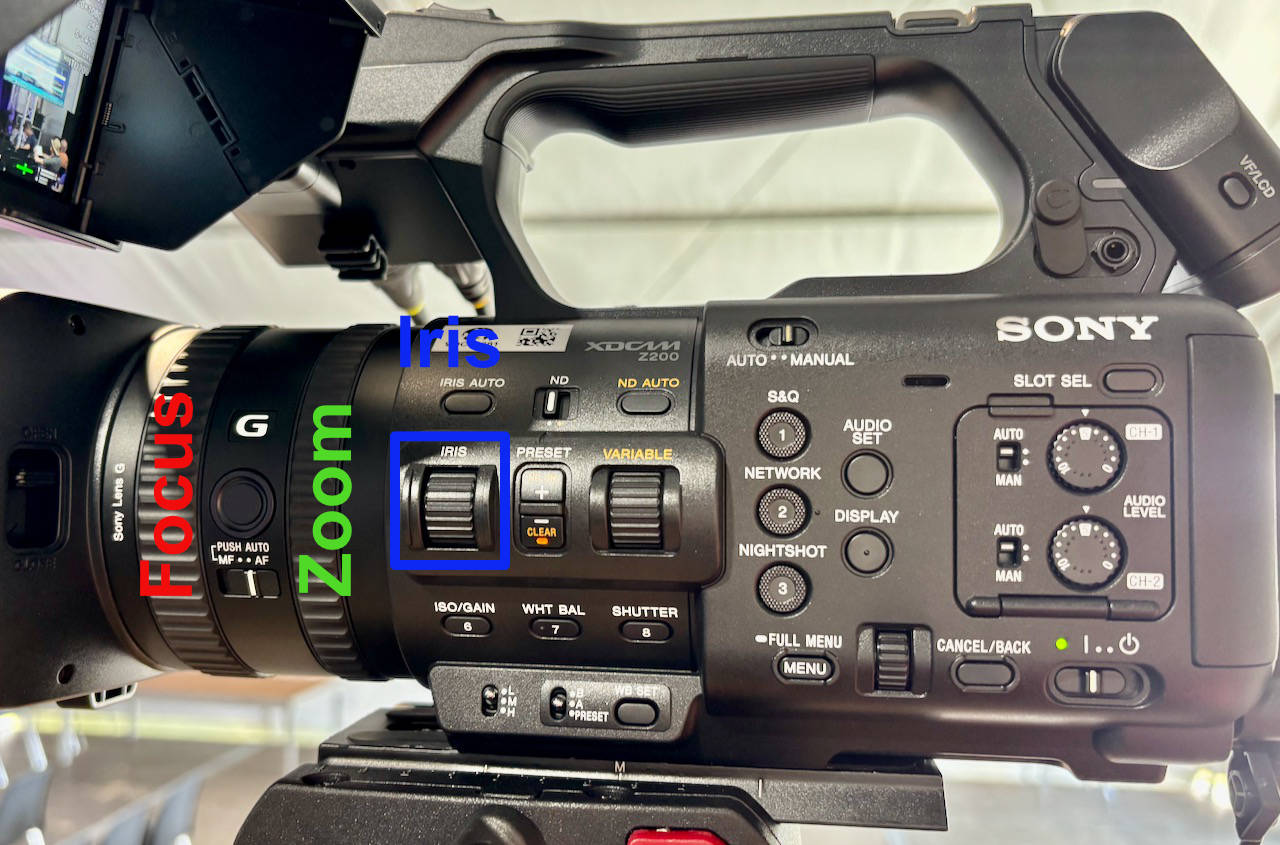
\includegraphics[width=0.9\textwidth]{images/sony-side-annotated.jpg}
		\caption{Sony Cam}
	\end{figure}
		\column{0.5\textwidth}
		Cameras are in manual mode because of difficult lighting situation.
		\begin{description}
			\item[Left Ring/red] Focus - control sharpness of the image.
			\item[MF/AF Selector] Auto Focus - always on.
			\item[Middle Ring/green] Zoom - vary the focal length.
			\item[Right Ring/blue] Iris - adjust according to lighting situation.
		\end{description}
	\end{columns}
  If there is anything wrong, contact C3VOC helpdesk.
\end{frame}

\begin{frame}{Zoom Control Sony}
	\begin{columns}[T,onlytextwidth]
		\column{0.5\textwidth}
	\begin{figure}
		\centering
		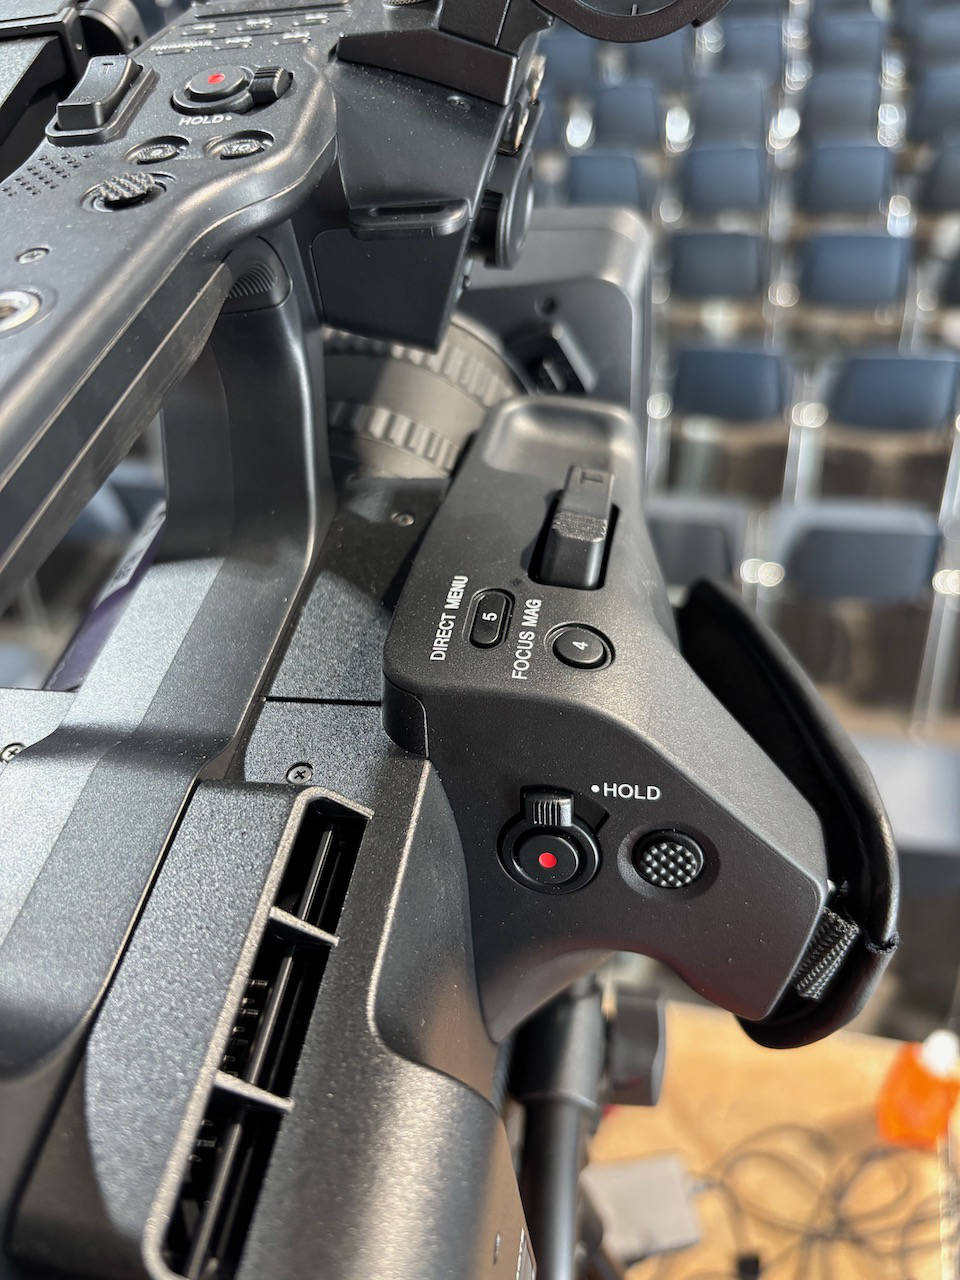
\includegraphics[width=0.99\textwidth]{images/sony-zoom.jpg}
		\caption{Sony Cam}
	\end{figure}
		\column{0.5\textwidth}
		\begin{itemize}
			\item For smooth zoom use the zoom buttons.
			\item Gentle touch $\Rightarrow$ slow zoom
		\end{itemize}
	\end{columns}
\end{frame}

\begin{frame}{Display Indicators Sony}
	\begin{columns}[T,onlytextwidth]
		\column{0.5\textwidth}
	\begin{figure}
		\centering
		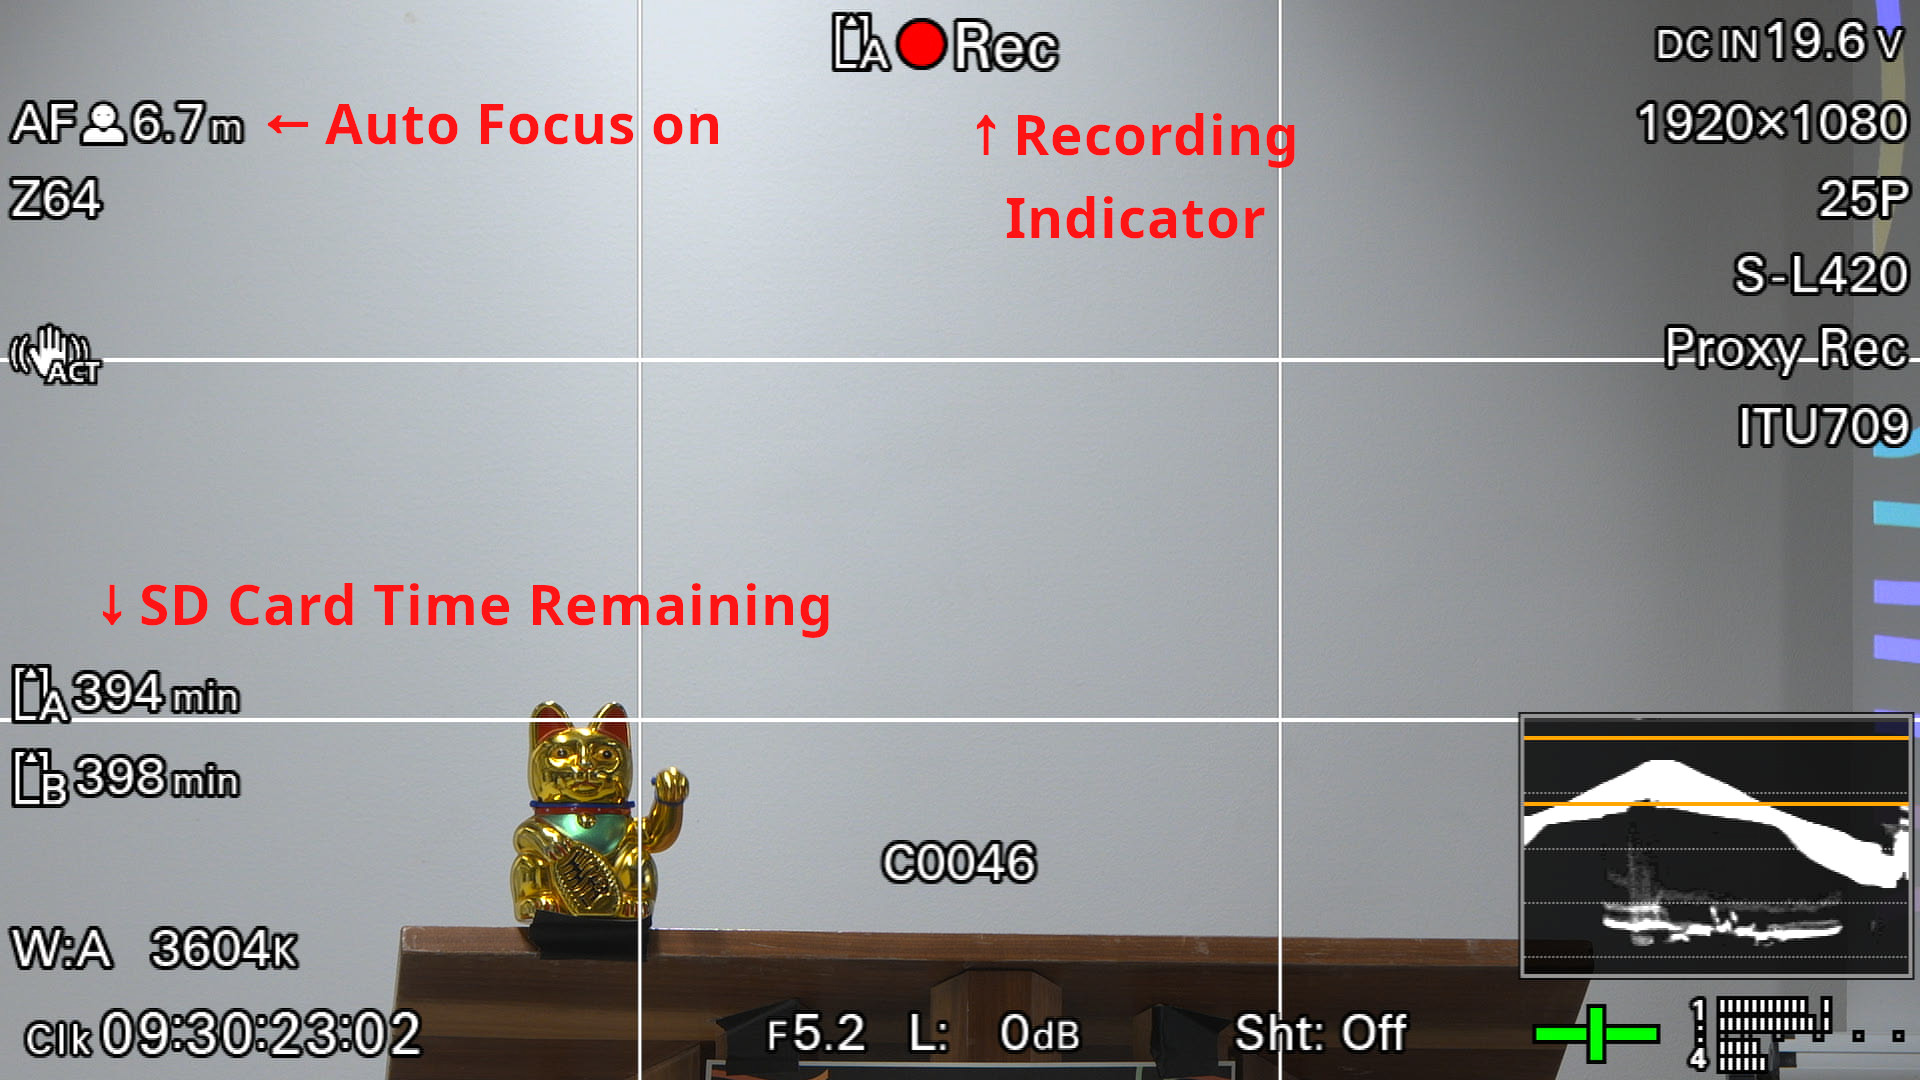
\includegraphics[width=0.9\textwidth]{images/sony-display-description.jpg}
		\caption{Sony Display Indicators}
	\end{figure}
		\column{0.5\textwidth}
		\begin{description}
			\item[Focal Indicator] Autofocus with face tracking is awesome!
			\item[Rec Indicator] The recording must always run, even during the break.
			\item[Remaining Time] More minutes remaining than the length of the next talk.
		\end{description}
		\metroset{block=fill}
		\begin{alertblock}{Alert}
			Alert the A/V-Technician if something's wrong.
		\end{alertblock}
	\end{columns}
\end{frame}
